\documentclass[usenames,dvipsnames]{beamer}
%\usetheme{}%\usecolortheme{}
\setbeamertemplate{navigation symbols}{}
\setbeamertemplate{section in toc}[sections numbered]
\setbeamertemplate{footline}[frame number]
\setbeamertemplate{caption}{\raggedright\insertcaption\par}

\usepackage[utf8]{inputenc}
\usepackage[T1]{fontenc}
\usepackage{lmodern}
\usepackage{appendixnumberbeamer}
\usepackage{multirow}
\usepackage{adjustbox}
\usepackage{tikz}
\usetikzlibrary{arrows,automata}

\newcommand{\textthemecolor}[1]{{\usebeamercolor[fg]{structure}#1}}
\newcommand{\policy}[1]{\texttt{\textbf{\textthemecolor{#1}}}}

% TODO:
%  - expliquer les différentes politiques de prédiction

\title{%
  {\bf WCET analysis} by {\bf Model Checking}
  \\ for a {\bf reasonnably complex system}}
\author{%
  {\bf Armel Mangean}$^2$
  \and Jean-Luc Béchennec$^1$
  \and Mikaël Briday$^3$
  \and Sébastien Faucou$^3$}
\institute{%
  $^1$CNRS, $^2$École Centrale de Nantes, $^3$Université de Nantes
  \\ LS2N}
\date{August 24, 2017}

% 20 min -> ~15 slides

\begin{document}

  \begin{frame}[plain,noframenumbering]
    \titlepage
    \begin{center}
      \small\emph{11th International Conference on Verification and Evaluation
        of Computer and Communication Systems}
    \end{center}
  \end{frame}

  \begin{frame}[plain,noframenumbering]
    \tableofcontents
  \end{frame}

  %%%
  
  \section{Introduction}
  \begin{frame}[plain,noframenumbering]
    \tableofcontents[currentsection]
  \end{frame}
  
  \subsection{Context}
  \begin{frame}
    \frametitle{\subsecname}
    \framesubtitle{Worst Case Execution Time (WCET) analysis}
    
    \begin{figure}
      \centering
      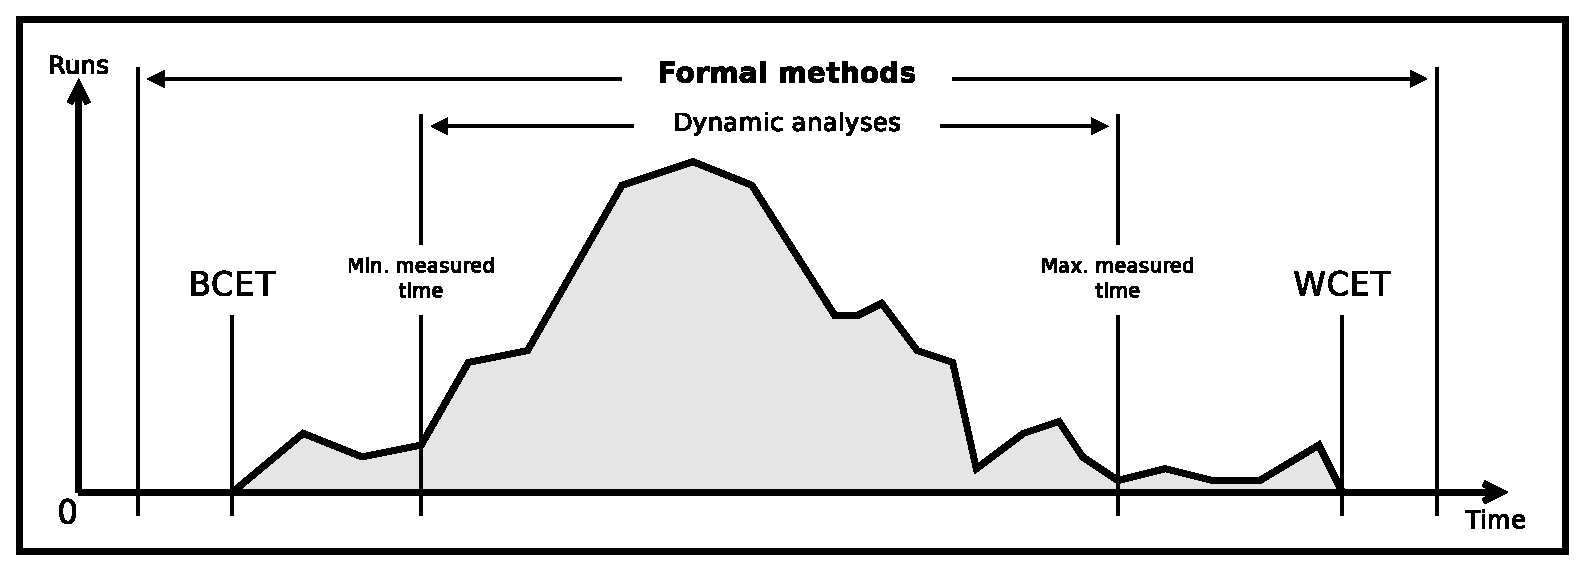
\includegraphics[width=\textwidth]{fig/wcet}
    \end{figure}

    %$\rightarrow$ for a \emph{reasonnably} complex system

    \begin{itemize}
      \item dynamic analyses produce under-approximations (unsafe)
      \item formal methods produce over-approximations (safe)
      \begin{itemize}
        \item[$\rightarrow$] effort to make precise over-approximations (sound)
      \end{itemize}
    \end{itemize}
  \end{frame}

  \begin{frame}
    \frametitle{\subsecname}
    \framesubtitle{WCET analysis by Model Checking}

    \begin{figure}
      \centering
      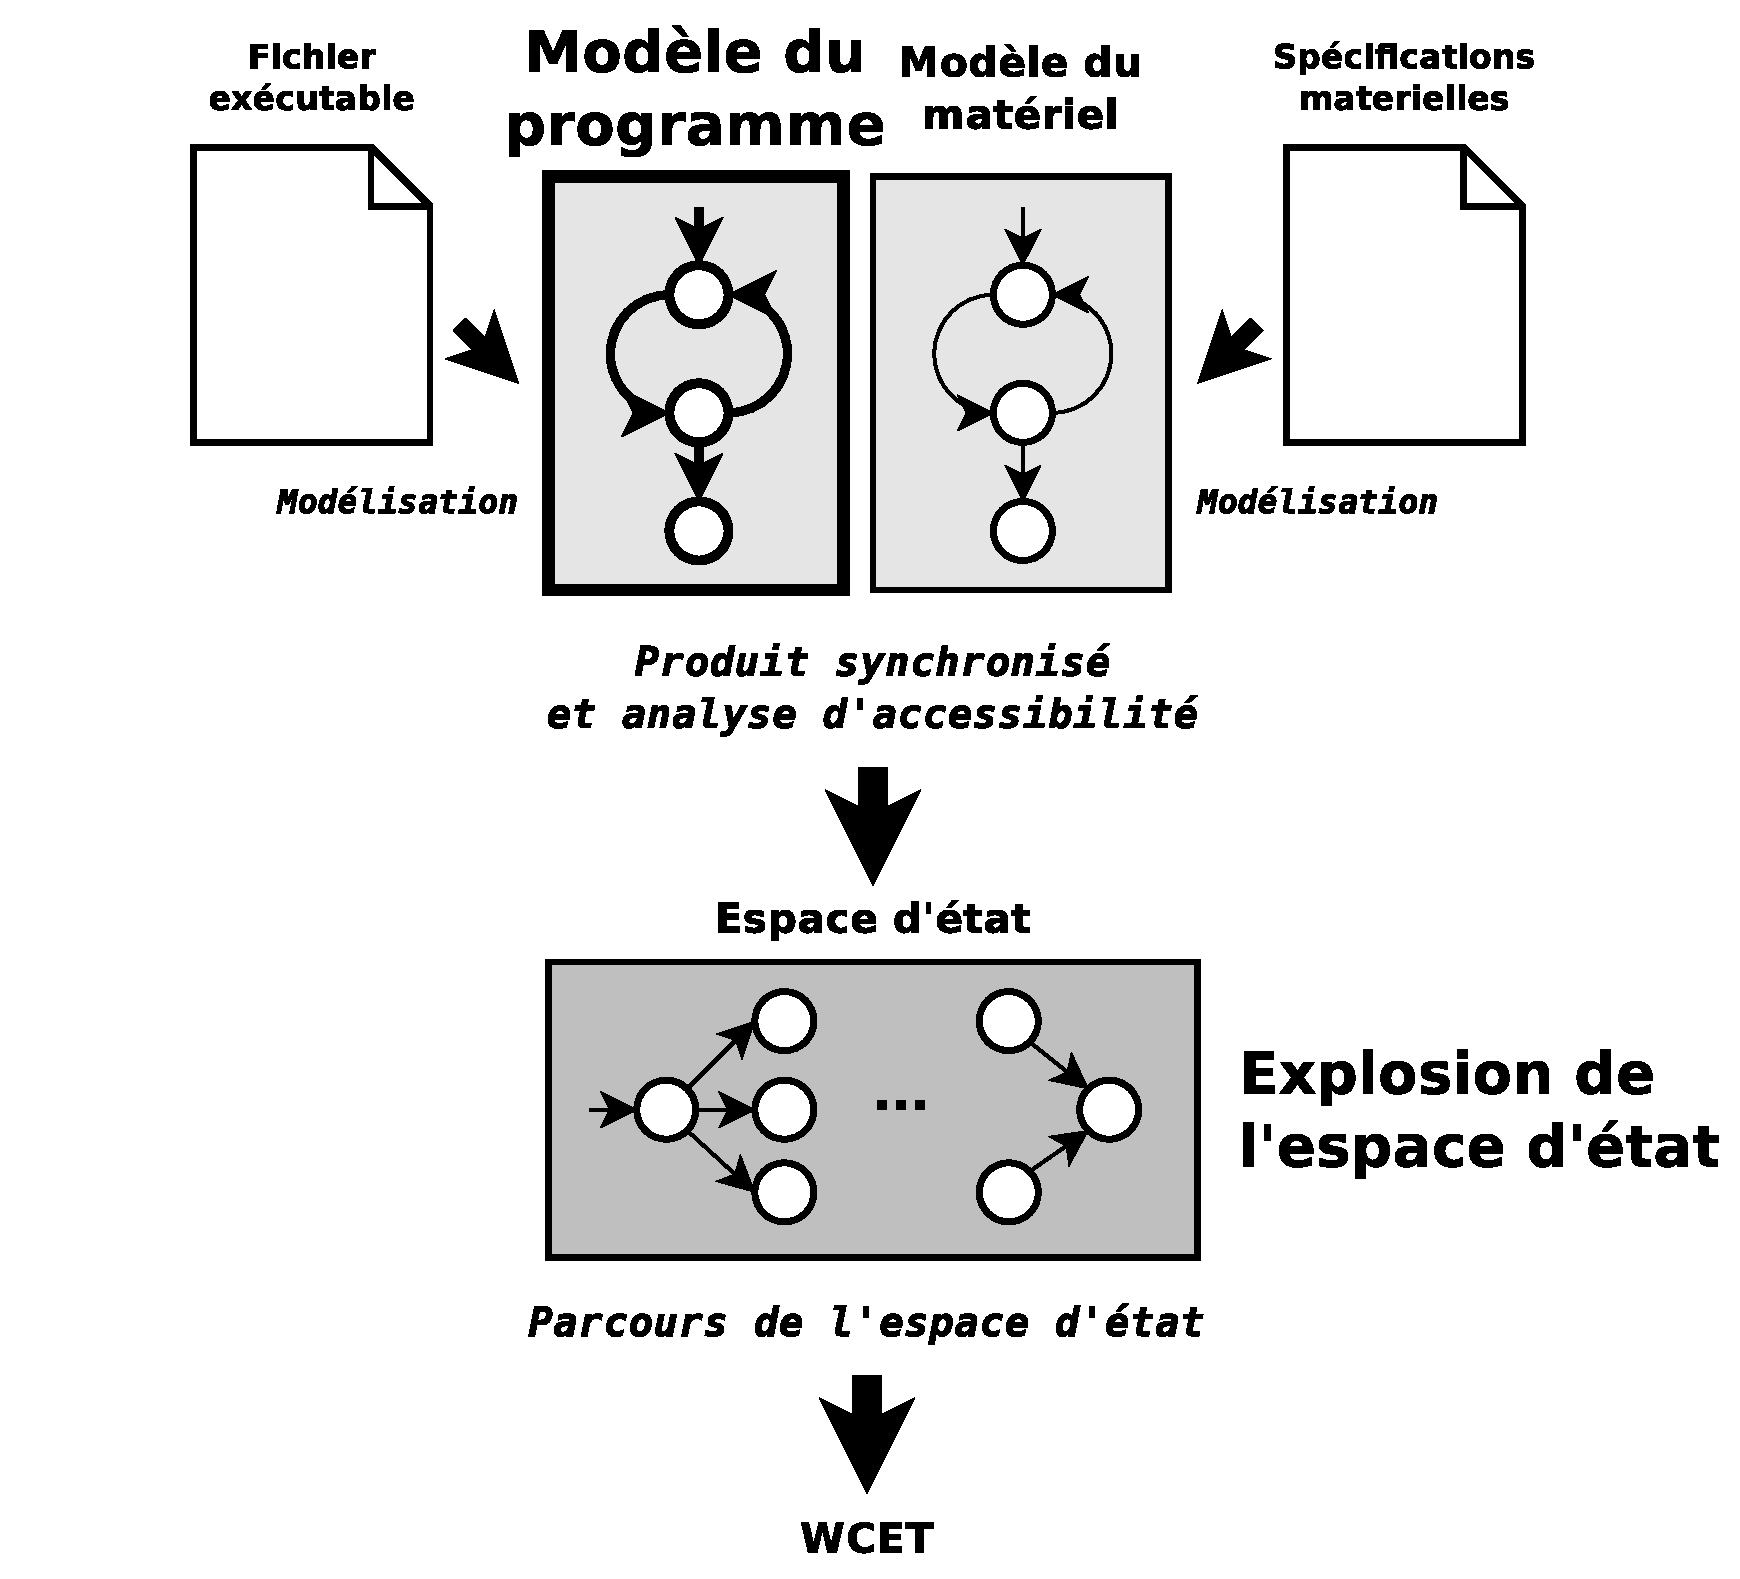
\includegraphics[height=.8\textheight]{fig/model-checking}
    \end{figure}
  \end{frame}

  \begin{frame}
    \frametitle{\subsecname}
    \framesubtitle{Advantages of Model Checking}
    \small
    
    \begin{description}[binary level]
      \item[witness] initial hardware and software configuration
      \item[tightness] \emph{e.g.} exact cache behavior with arbitrary replacement policies%, see~\cite{Metzner:2004}
        \begin{itemize} % infeasible with AI
          \item not only LRU nor PLRU
        \end{itemize}          
    \end{description}

    \vspace{1em}
    $\rightarrow$ infeasible with the most widely used formal approach

    \vspace{1em}
    \begin{description}[binary level]
      \item[modularity] network of timed automata
      \item[binary level] no high level source code analysis
        \begin{itemize}
          \item compiler independent
          \item avoid accumulation of approximations
      %    %\item no need for annotations
      %    %\item no problem induced by optimization options
        \end{itemize}            
    \end{description}
  \end{frame}
  
  \subsection{Motivation}
  \begin{frame}
    \frametitle{\subsecname}
    \framesubtitle{~}
    \small
      
    \begin{block}{Known limitations}
      \begin{itemize}
      \item suffer of the state space explosion%~\cite{Wilhelm:2004}
        \begin{itemize}
        \item[$\rightarrow$] focus on embedded microcontrollers and hard Real-Time % but thus precise
          \end{itemize}
      \end{itemize}
    \end{block}
    
    \vspace{1em}
    \begin{block}{Challenges}
      \begin{itemize}
        \item model programs %~\cite{Mangean:2016} (previous work)
        \item {\bf model hardware components} % efficiently wrt. the state space explosion problem
        \item {\bf investigate feasibility of WCET analysis by Model Checking}
      \end{itemize}
    \end{block}
  \end{frame}

  %%%

  \section{Modeling a reasonnably complex system}
  \begin{frame}[plain,noframenumbering]
    \tableofcontents[currentsection]
  \end{frame}

  \begin{frame}
    \frametitle{\secname}
    \small

    \begin{block}{The hardware plateform}
      $\rightarrow$ based on the \textsc{Power} e200z4 microcontroller
    \end{block}

    \begin{block}{\textsc{Uppaal} timed automata}
      \begin{itemize}
        \item timing behavior modeled as
        \begin{itemize}
          \item \textcolor{Green}{guards} on clocks and synchronisation \textcolor{cyan}{channels} on transitions
          \item clocks \textcolor{purple}{invariants} on locations
        \end{itemize}
        \item functionnal behavior modeled as
        \begin{itemize}
          \item \textcolor{Green}{guards} and \textcolor{blue}{actions} on transitions
          \item[$\rightarrow$] data structures manipulation 
        \end{itemize}
      \end{itemize}
    \end{block}
  \end{frame}

  \subsection{Modeling the pipeline}
  \begin{frame}
    \frametitle{\subsecname}
    %\framesubtitle{Functional behavior}
    \small

    \begin{columns}
    \begin{column}{.66\linewidth}
    \begin{itemize}
      \vspace{-3em}
      \item a classic 5-stage pipeline
      \begin{itemize}
        \item fetch~(\policy{F}), decode~(\policy{D}), execute~(\policy{E}), memory~(\policy{M}) and writeback~(\policy{W})
        \item 5-entry array of pipeline stage
      \end{itemize}

      \vspace{3em}
      \item an instruction buffer (\policy{IBuff})
      \begin{itemize}
        \item between the \policy{F} and \policy{D} stages
        \item 8-entry array of instruction
      \end{itemize}
    \end{itemize}
    \end{column}

    \begin{column}{.33\linewidth}
        \begin{figure}
          \centering
          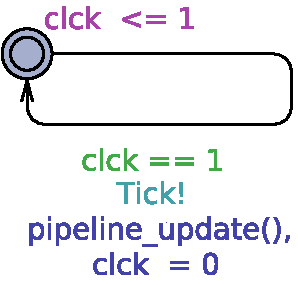
\includegraphics[scale=.45]{fig/pipeline}
          \caption{Pipeline model}
        \end{figure}

        \begin{figure}
          \centering
          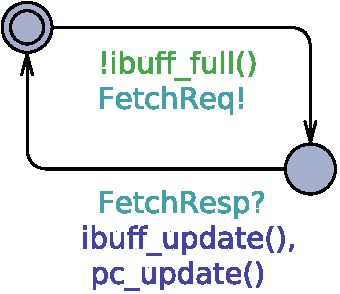
\includegraphics[scale=.45]{fig/incu}
          \caption{Instruction Buffer model}
        \end{figure}
    \end{column}
    \end{columns}
  \end{frame}

  \subsection{Modeling the branch prediction unit}
  \begin{frame}
    \frametitle{\subsecname}
    \framesubtitle{~}
    \small

    \begin{itemize}
      \item a branch target buffer (\policy{BTB})
      \begin{itemize}
        \item used at \policy{F} stage
        \item 8-entry buffer, each containing
      \begin{itemize}
        \item a branch instruction address
        \item a branch instruction target
        \item a 2-bit saturating counter 
      \end{itemize}
      \end{itemize}
    \end{itemize}

    \pause
    \vspace{1em}
    \begin{figure}
    \centering
    \begin{adjustbox}{width=\textwidth,keepaspectratio}
      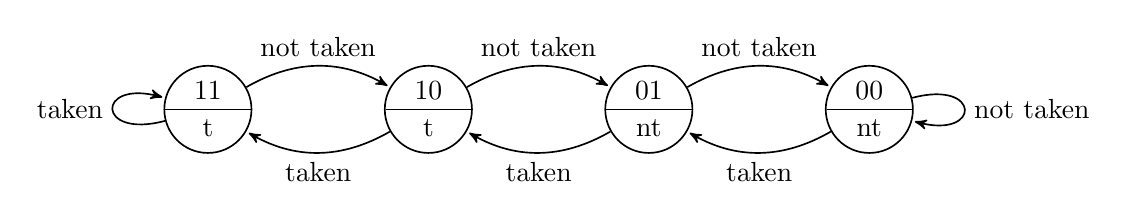
\begin{tikzpicture}[->,>=stealth',shorten >=1pt,auto,node distance=2.8cm,
    semithick,state/.style=state with output]
  \tikzstyle{every state}=[fill=none,draw=black,text=black]

  \node[state]                                     (WNT) {$01$ \nodepart{lower} nt};
  \node[state]                                     (NT) [right of=WNT] {$00$ \nodepart{lower} nt};
  \node[state]                                     (WT) [left of=WNT] {$10$ \nodepart{lower} t};
  \node[state]                                     (T)  [left of=WT] {$11$ \nodepart{lower} t};

  \path (NT)    edge [bend left]  node {taken} (WNT)
        (NT)    edge [loop right] node {not taken} (NT)
        (WNT)   edge [bend left]  node {not taken} (NT)
        (WNT)   edge [bend left]  node {taken} (WT)
        (WT)    edge [bend left]  node {not taken} (WNT)
        (WT)    edge [bend left]  node {taken} (T)
        (T)     edge [bend left]  node {not taken} (WT)
        (T)    edge [loop left]  node {taken} (T);
\end{tikzpicture}

    \end{adjustbox}
      \caption{A 2-bit saturating counter. \texttt{t}: taken; \texttt{nt}: not-taken}
    \end{figure}
  \end{frame}

  \begin{frame}
    \frametitle{\subsecname}
    \framesubtitle{Branch prediction policies}
    \small

    \begin{block}{Static only policies (at \policy{D} stage)}
      \begin{itemize}
        \item Always Not-taken (\policy{AN})
        \item Backward Taken / Forward Not-taken (\policy{BT/FN})
        \begin{description}[Forward Not-taken]
          \item[Backward Taken] Loop related
          \item[Forward Not-taken] Else clause related
        \end{description}
      \end{itemize}
    \end{block}

    \begin{block}{Dynamic + static and  policy (at \policy{F} and \policy{D} stages)}
      \begin{itemize}
        \item \policy{BT/FN} and use a the BTB (\policy{BT/FN+BTB})
      \end{itemize}
    \end{block}
  \end{frame}

  \subsection{Modeling the memory hierarchy}
  \begin{frame}
    \frametitle{\subsecname}
    \framesubtitle{~}

    \begin{itemize}
      \item an instruction cache (\policy{ICache})
      \begin{itemize}
        %\item 2 or 4-ways set associative
        \item model of the exact cache behavior
        \item pseudorandom remplacement policy
        \begin{itemize}
          %\item 1 or 2 bits identify the way of the line to replace
          \item[$\rightarrow$] infeasible with the most widely used formal approach
       \end{itemize}
      \end{itemize}

      \pause
      \vspace{1em}
      \item a instruction cache fill buffer (\policy{FillBuff})
      \begin{itemize}
        \item buffer used to refill a cache line after a cache miss
        %\item copied to the ICache when full
      \end{itemize}

      \pause
      \vspace{1em}
      \item Burst-mode memory access (\policy{Burst})
      \begin{itemize}
        \item transfer data from RAM to fill buffer
        \item 4 consecutive 2-instruction reads
        \item lowering the overhead
      \end{itemize}
    \end{itemize}
  \end{frame}

  \begin{frame}
    \frametitle{\subsecname}
    \framesubtitle{~}

    \begin{figure}
      \centering
      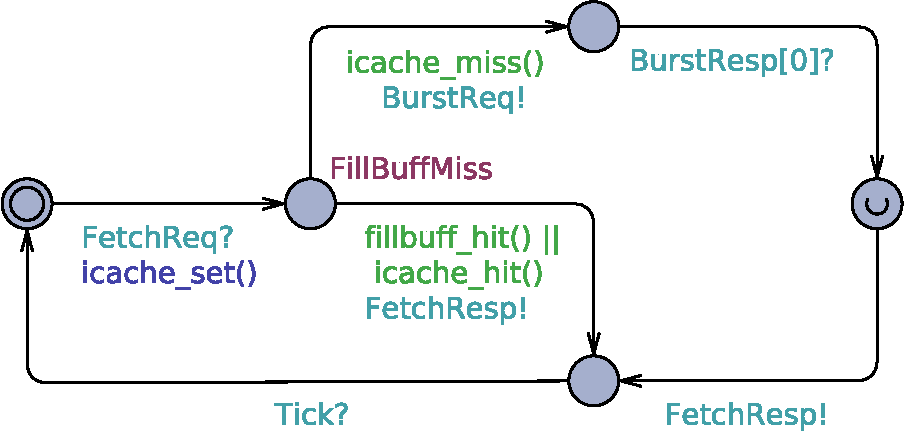
\includegraphics[scale=.45]{fig/icache}
      \caption{Instruction Cache model}
    \end{figure}
  \end{frame}

  \subsection{Modeling programs}
  \begin{frame}
    \frametitle{\subsecname}
    \framesubtitle{Introducing Program Slicing}

    \begin{figure}
      \centering
      \begin{overlayarea}{\textwidth}{\textheight}
        \only<1>{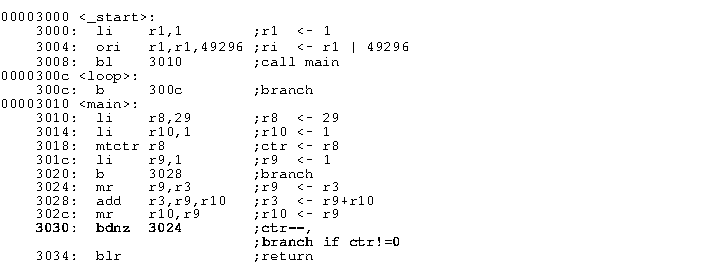
\includegraphics[scale=1.4]{fig/fibcallO2-01.pdf}}
        \only<2>{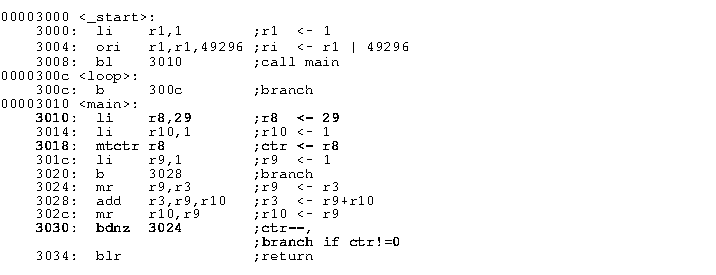
\includegraphics[scale=1.4]{fig/fibcallO2-02.pdf}}
        \begin{center}
          $\rightarrow$ for the \emph{slicing criterion} $C = ( 3030, \{ctr\} )$
        \end{center}
      \end{overlayarea}
    \end{figure}
  \end{frame}

  \begin{frame}
    \frametitle{\subsecname}
    \framesubtitle{Abstracting program models with Program Slicing}

    \begin{center}
      $\rightarrow$ Need for time accurate abstract program models 
    \end{center}

    \begin{block}{}%From previous work}%~\cite{Mangean:2016}}
      \begin{itemize}
        \item abstract models must contain all paths from original model
          \begin{itemize}
            \item ie. contain all control instructions and their dependencies
          \end{itemize}
        
        \vspace{1em}
        \item Program Slicing can be used to gather these instructions
          \begin{itemize}
            \item a slicing criterion is chosen wrt. the previous constraint
          \end{itemize}
      \end{itemize}
    \end{block}
  \end{frame}

  \begin{frame}
    \frametitle{\subsecname}
    \framesubtitle{An abstract program model}
    \small

    \begin{figure}
      \centering
      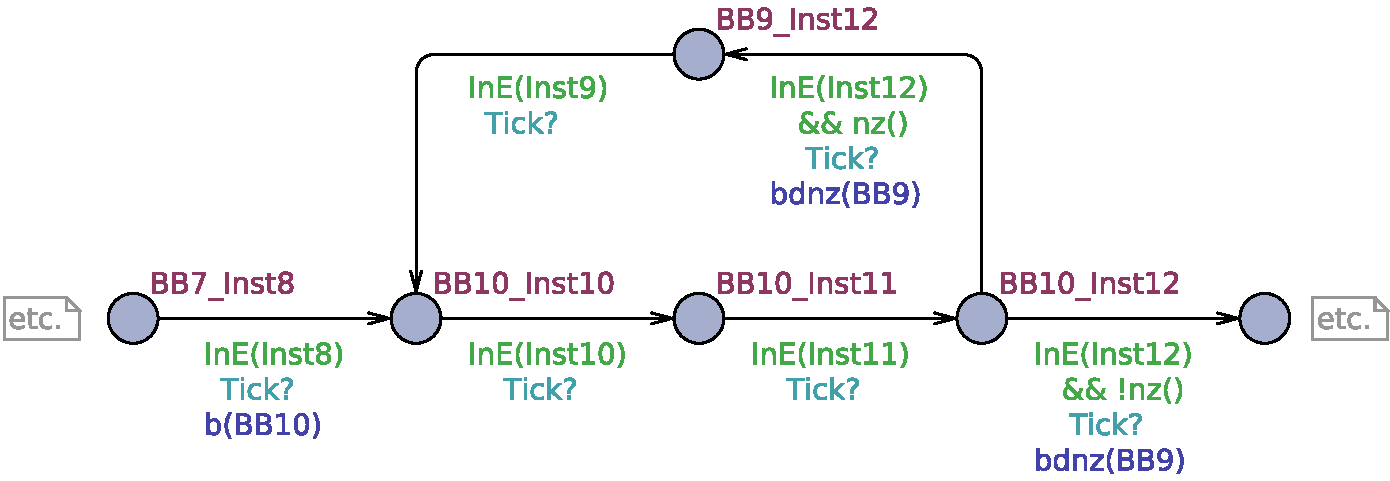
\includegraphics[scale=.45]{fig/program}
    \end{figure}
    \begin{itemize}
      \item \textcolor{Green}{guards} and \textcolor{cyan}{channels} model the timing behavior of \textbf{all} instructions
      \vspace{-.4em}\item \textcolor{blue}{actions} model the functionnal behavior of \textbf{sliced} instructions
    \end{itemize}
  \end{frame}

  \begin{frame}
    \frametitle{\secname}
    \framesubtitle{WCET analysis by Model Checking}
    \small

    \begin{figure}
      \centering
      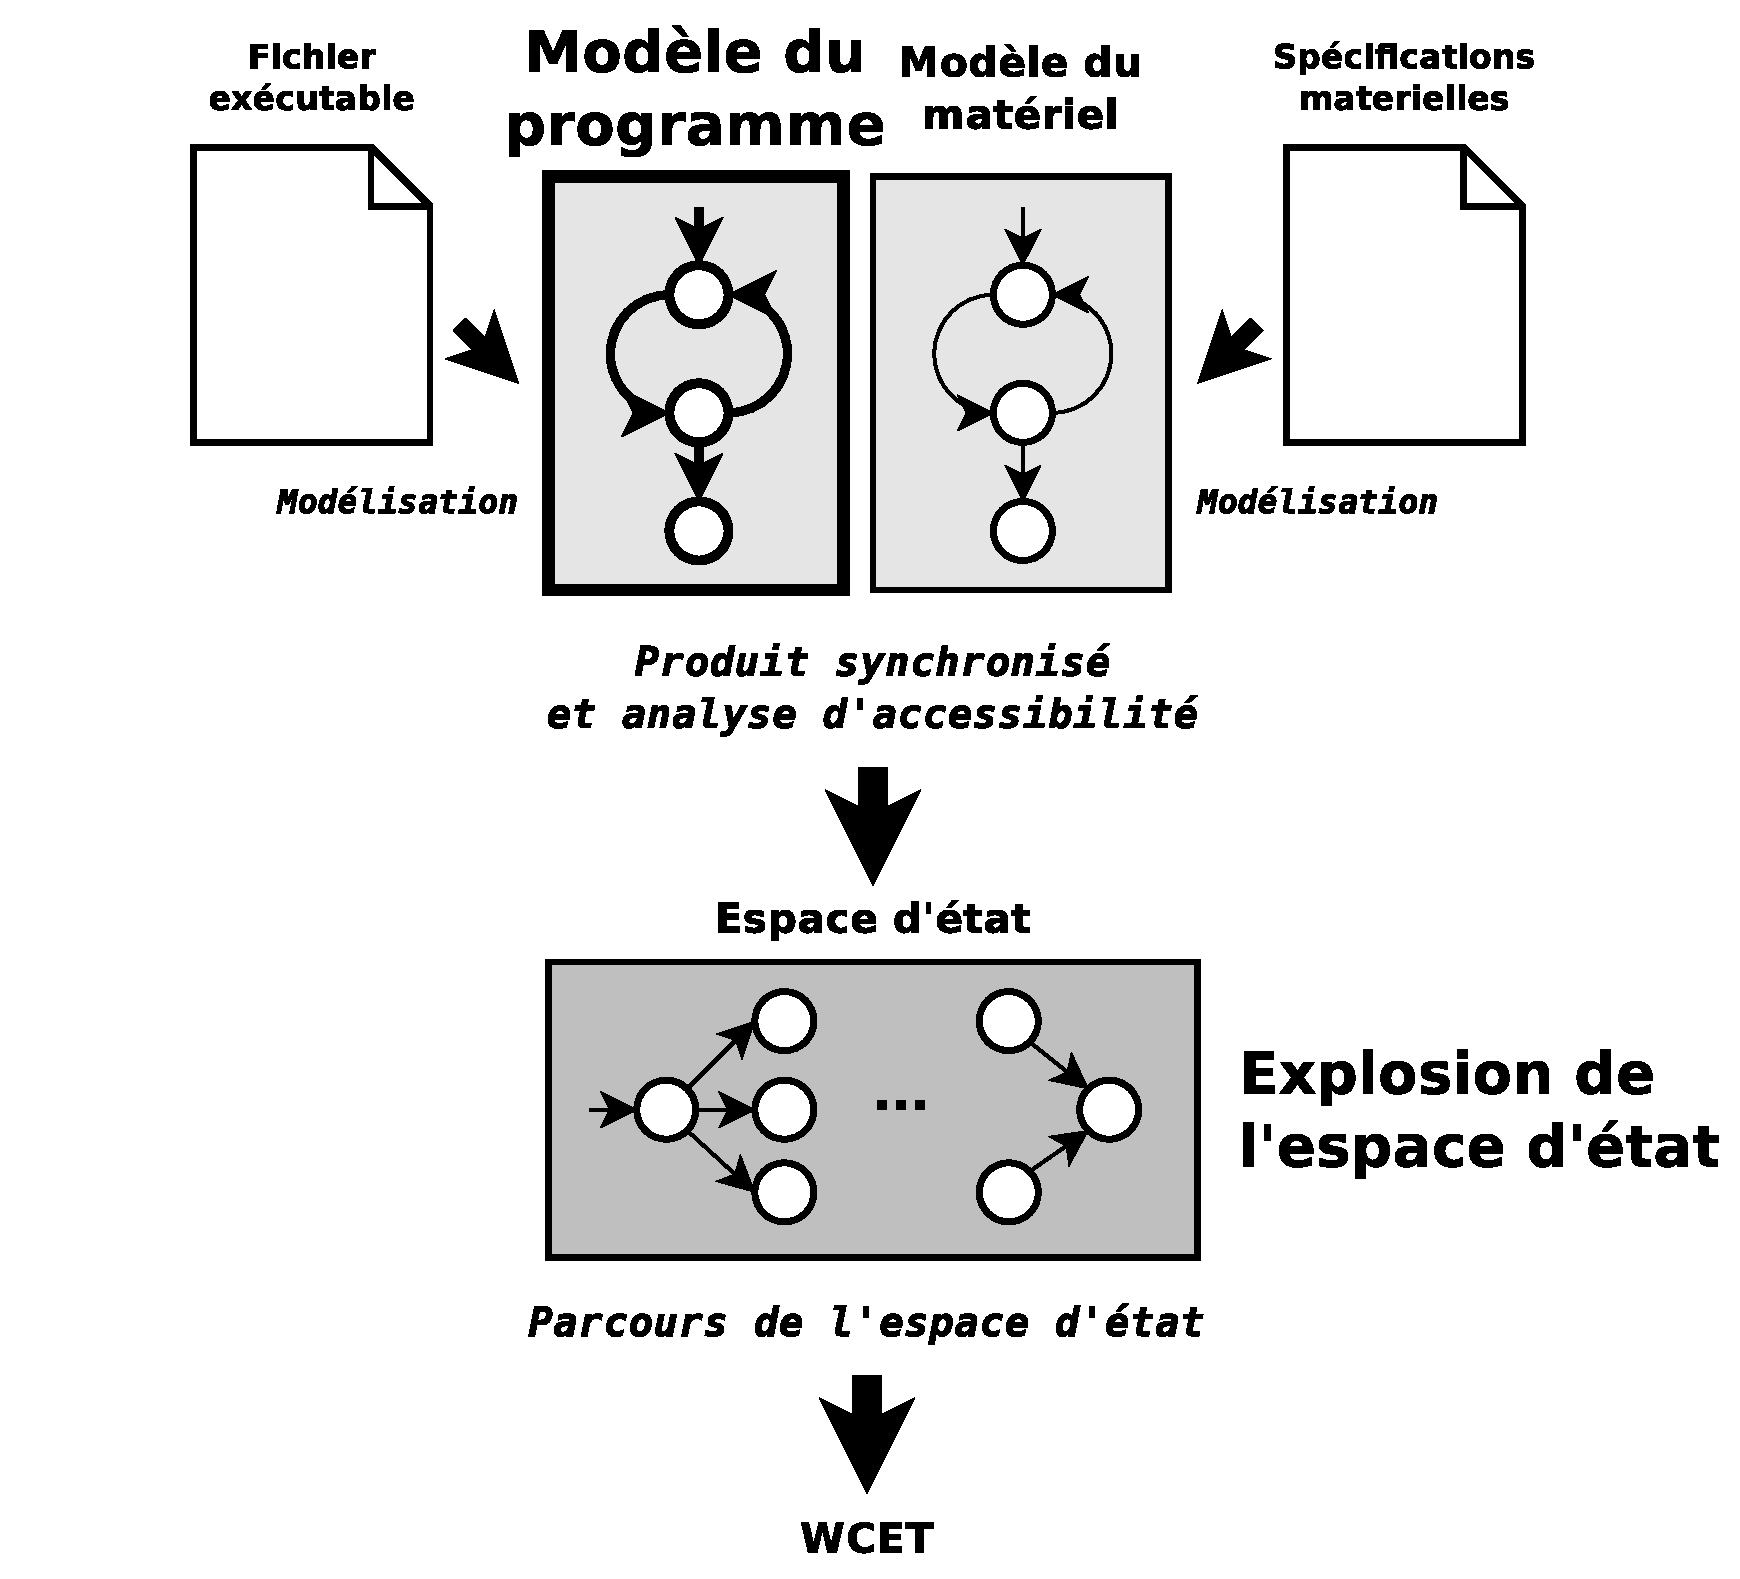
\includegraphics[height=.8\textheight]{fig/model-checking}
    \end{figure}
  \end{frame}

  %%%
  
  \section{Experimental results}
  \begin{frame}[plain,noframenumbering]
    \tableofcontents[currentsection]
  \end{frame}
  
  \subsection{Methodology}
  \begin{frame}
    \frametitle{\subsecname}
    \framesubtitle{~}
    \small

    \begin{itemize}
      \item use of the \textsc{Mälardalen} benchmark collection%~\cite{Gustafsson:2010}
      \item excluding programs containing % 16 out of the 35
        \begin{itemize}
          \item \textbf{recursive programs} % impossible w/ MC
          \item stack dependent instructions % not (yet) implemented
          \item switch-case statements and function pointers % whereas it's a closed issue (not implemented)
          \item floating-point arithmetic % missing in the PowerPC HADL file 
        \end{itemize}

      \vspace{1em}
      \item run for 3 branch prediction policies (\policy{AN}, \policy{BT/FN} and \policy{BT/FN+BTB})

      %\item compiled with \textsc{Gcc} 5.3.1 with \texttt{-O1} and \texttt{-O2}
      %\item run on an Intel Core i7-3770 (4 cores, 3.4GHz),
      %   \\ 8GiB RAM, Debian 9 (64-bit, Linux 4.9)
    \end{itemize}
  \end{frame}
  
  \subsection{Results}
  \begin{frame}
    \frametitle{\subsecname}
    \framesubtitle{Resources consumption}
    \small

    \begin{table}
      \scriptsize
      \centering
      \begin{tabular}{|l||r|r|r|r|}
                                                                              \hline
        Program & Opt. & States & Memory (MiB) & CPU time (s.) \tabularnewline\hline
                                                                              \hline
        bs               & {\tt -O2}  &    451 &  11.855 & 0.000   \tabularnewline\hline
        bs               & {\tt -O1}  &    586 &  12.386 & 0.010   \tabularnewline\hline
        fibcall          & {\tt -O2}  &    590 &  10.742 & 0.000   \tabularnewline\hline
        janne\_complex   & {\tt -O2}  &    594 &  12.277 & 0.000   \tabularnewline\hline
        janne\_complex   & {\tt -O1}  &    779 &  12.218 & 0.010   \tabularnewline\hline
     %% fibcall          & -O1  &    949 &  11.820 & 0.010   \tabularnewline\hline
     %% insertsort       & -O2  &   2995 &  13.785 & 0.020   \tabularnewline\hline
     %% expint           & -O2  &   4118 &  13.535 & 0.040   \tabularnewline\hline
     %% expint           & -O1  &   5967 &  21.714 & 0.040   \tabularnewline\hline
     %% fdct             & -O1  &   6823 &  23.246 & 0.050   \tabularnewline\hline
     %% fdct             & -O2  &   7080 &  24.933 & 0.050   \tabularnewline\hline
     %% jfdctint         & -O1  &  11121 &  30.894 & 0.100   \tabularnewline\hline
     %% cnt              & -O2  &  11279 &  29.789 & 0.110   \tabularnewline\hline
     %% ud               & -O2  &  11305 & 479.785 & 0.380   \tabularnewline\hline
     %% jfdctint         & -O2  &  11349 &  33.003 & 0.100   \tabularnewline\hline
     %% bsort100         & -O2  &  11982 &  27.214 & 0.130   \tabularnewline\hline
     %% prime            & -O2  &  12056 &  24.964 & 0.080   \tabularnewline\hline
     %% prime            & -O1  &  12072 &  25.937 & 0.080   \tabularnewline\hline
     %% bsort100         & -O1  &  12457 &  28.507 & 0.130   \tabularnewline\hline
     %% ns               & -O2  &  31229 &  39.332 & 0.030   \tabularnewline\hline
                                                                            \hline
        ...              & ...  &    ... &     ... &   ...   \tabularnewline\hline
                                                                            \hline
        ns               & {\tt -O1}  &  32482 &  43.910 & 0.250   \tabularnewline\hline
        crc              & {\tt -O2}  & 144653 & 483.164 & 1.570   \tabularnewline\hline
        crc              & {\tt -O1}  & 157612 & 537.156 & 1.600   \tabularnewline\hline
        fir              & {\tt -O2}  & 692704 & 594.152 & 4.430   \tabularnewline\hline
        {\bf fir} & {\bf\texttt{-O1}}  & {\bf 728321} & {\bf 640.261} & {\bf 4.770}   \tabularnewline\hline
      \end{tabular}
    \end{table}

    \begin{center}
      Resources consumption for the \policy{AN} policy \\
      (ordered by number of states)
    \end{center}
  \end{frame}

  \begin{frame}
    \frametitle{\subsecname}
    \framesubtitle{State spaces comparison}

    \small
    \begin{figure}
      \centering
      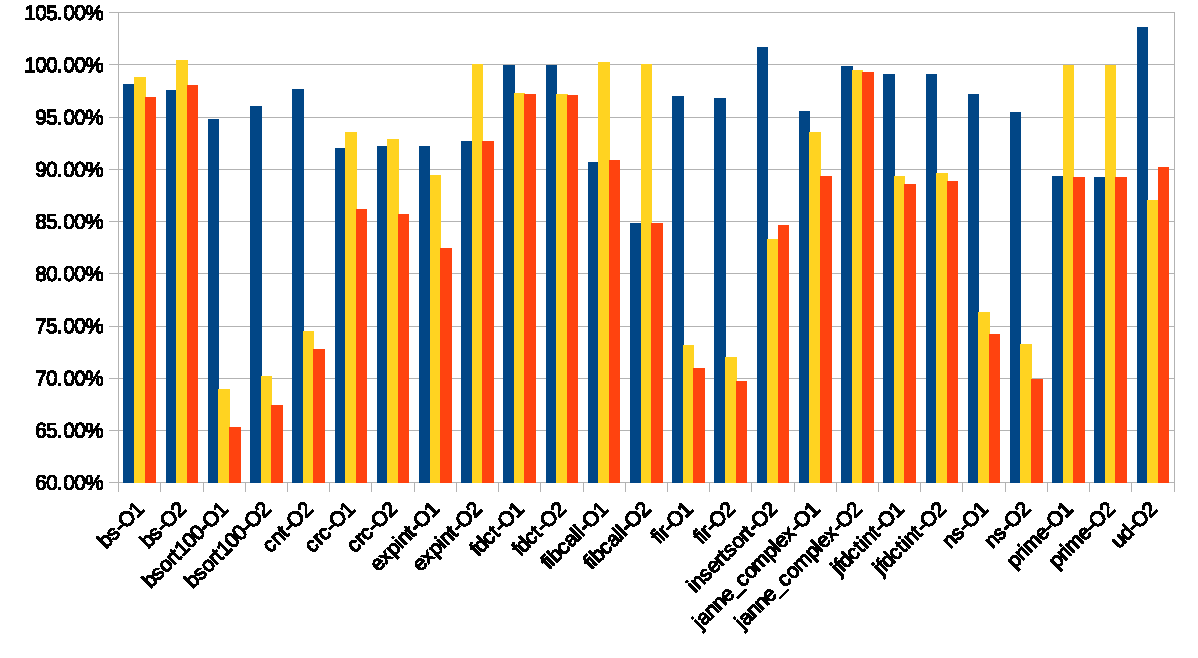
\includegraphics[width=\linewidth]{fig/statespace_ratios}
    \end{figure}

    \begin{description}
      \vspace{-2.em}\item[\textcolor{Blue}{Blue}] ratios for \policy{BT/FN} over \policy{AN}
      \vspace{-.5em}\item[\textcolor{Dandelion}{Yellow}] ratios for \policy{BT/FN+BTB} over \policy{BT/FN}
      \vspace{-.5em}\item[\textcolor{red}{Red}] ratios for \policy{BT/FN+BTB} over \policy{AN}
    \end{description}

    %(for \texttt{bsort-O1}, BTFN+BTB state space is 65\% of the AN state space)
  \end{frame}
  
  \begin{frame}
    \frametitle{\subsecname}
    \framesubtitle{Analysis}
    \small

    \begin{block}{On state spaces}
    \begin{itemize}
      \item in average, \policy{AN} > \policy{BT/FN} > \policy{BT/FN+BTB}
      \item \textthemecolor{counter intuitive:} more complex model produce smaller state space
      \begin{itemize}
        \item[$\rightarrow$] less mispredictions implies less states
      \end{itemize}
    \end{itemize}
    \end{block}

    \pause
    \begin{block}{On WCET upper bounds}
    \begin{itemize}
      \item no policy strictly dominates another
      \item \textthemecolor{counter intuitive:} more complex policies occasionally produce \\
       \hspace{7.2em} bigger WCET
      \begin{itemize}
        \item[$\rightarrow$] depends on interaction of the software and hardware
        \item[$\rightarrow$] no worst policy implies to test for all policies
      \end{itemize}
    \end{itemize}
    \end{block}
  \end{frame}

  %%%
  
  \section{Future work}
  \begin{frame}[plain,noframenumbering]
    \tableofcontents[currentsection]
  \end{frame}
  
  \begin{frame}
    \frametitle{\secname}

    \begin{itemize}
      \item support a wider range of binaries
      \begin{itemize}
        \item use the TACLe benchmark collection
      \end{itemize}

      \vspace{1em}
      \item model a MPC5643L microprocessor % and closer to real hardware
      %% \begin{itemize}
      %%   \item two e200z4 cores %(closer to real)
      %%   \item a XBAR crossbar switch
      %%     \begin{itemize}
      %%       \item multiple masters / multiple slaves
      %%       \item per slave policy (Fixed Priority or Round-Robin)
      %%     \end{itemize}
      %% \end{itemize}
      \begin{itemize}
        \item each e200z4 core as 2-way superscalar
        \item multicore (two e200z4 cores) %(closer to real)
        \item a XBAR crossbar switch
        \item make use of undeterminism on initial hardware state
      \end{itemize}

      \vspace{1em}
      \item make WCET analyses of parallel programs
      \begin{itemize}
        \item compare results to real life execution % microbenchmarking 
      \end{itemize}
    \end{itemize}
  \end{frame}

  %%%

  \section*{Conclusion}
  \begin{frame}
    \frametitle{\secname}
    \small

    \begin{block}{A reasonnably complex system}
    \begin{itemize}
      \item abstract program models % based on Malardalen
      \item model complex hardware components
      \begin{itemize}
        \item 5-stage pipeline with an instruction prefecth buffer
        \item a branch prediction unit with 3 policies
        \item instruction cache
      \end{itemize}
      \item representative of a safety critical embedded control system

    \end{itemize}
    \end{block}
    
    \pause
    \begin{block}{WCET analysis by Model Checking}
    \begin{itemize}
      \item allows to explore only feasible traces of the system
      \begin{itemize}
        \item actual sequence of memory access requests
        \item exact pipeline stall states
      \end{itemize}
      \item promising results concerning the scalability of the approach
      %\item need for more developpment and experiments to identify limits
    \end{itemize}
    \end{block}
  \end{frame}
  
  %%%
  
  %\appendix
  %\section{References}
  %\begin{frame}%[allowframebreaks]
  %  \frametitle{\secname}
  %  \tiny
  %  
  %  \bibliographystyle{plain}
  %  \bibliography{src/refs}
  %cite\end{frame}

\end{document}

